\chapter{Preparation}
\par In this chapter, we will introduce some preparation work for the proposed system. At first, we employed the OpenPose library\cite{cao2017realtime} to extract the orator's joint data from past speech 2D video, and we will introduce the OpenPose library in section 1. Then we set up a Microsoft Kinect for Windows Version device\cite{Shotton2011} to extract the trainee's joint data in training, and we will introduce the Kinect camera in section 2. To evaluate the effectiveness of the proposed system, we need to know how to evaluate a presentation, and we will introduce some evaluation points of a presentation.
\section{Joint Data Extraction Method (2D)}
We employed the OpenPose library to extract the orator's joint data from 2D speech video\cite{cao2017realtime}. OpenPose is a library for real-time multi-person keypoint (Figure \ref{fig:Keypoints detected by OpenPose}) detection and multi-threading written in C++ using OpenCV and Caffe\cite{Jia2014}. OpenPose can detect human body, hand and facial keypoionts on single images. In addition, the system computational performance on body keypoint estimation is invariant to the number of detected people in the image.
\begin{figure}[htbp]
\centering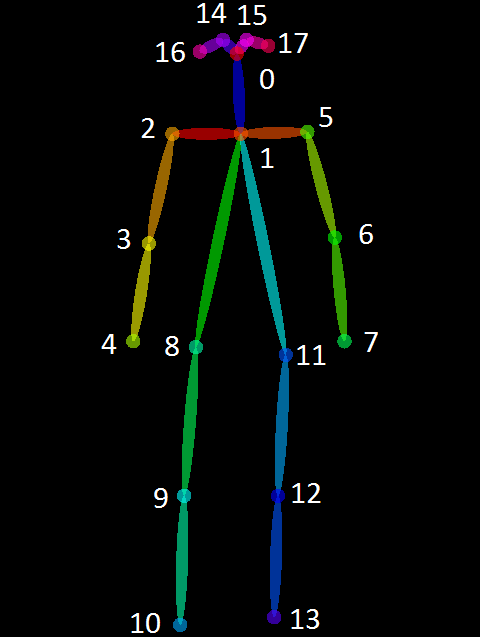
\includegraphics[scale=0.55]{./img/keypoints_openpose.png}
\caption{Keypoints detected by OpenPose}\label{fig:Keypoints detected by OpenPose}
\end{figure}

\par OpenPose is a kind of Convolutional Pose Machine (CPM) that use Convolutional Neural Networks (CNNs) to detect the human joint data from 2D image or video. CPMs consist of a sequenece of convolutional networks that repeatedly produce 2d belief maps for the location of each part (Figure \ref{fig:eft}). At each stage, image features and belief maps produced by the previous stage are used as input.
\begin{figure}[htbp]
\centering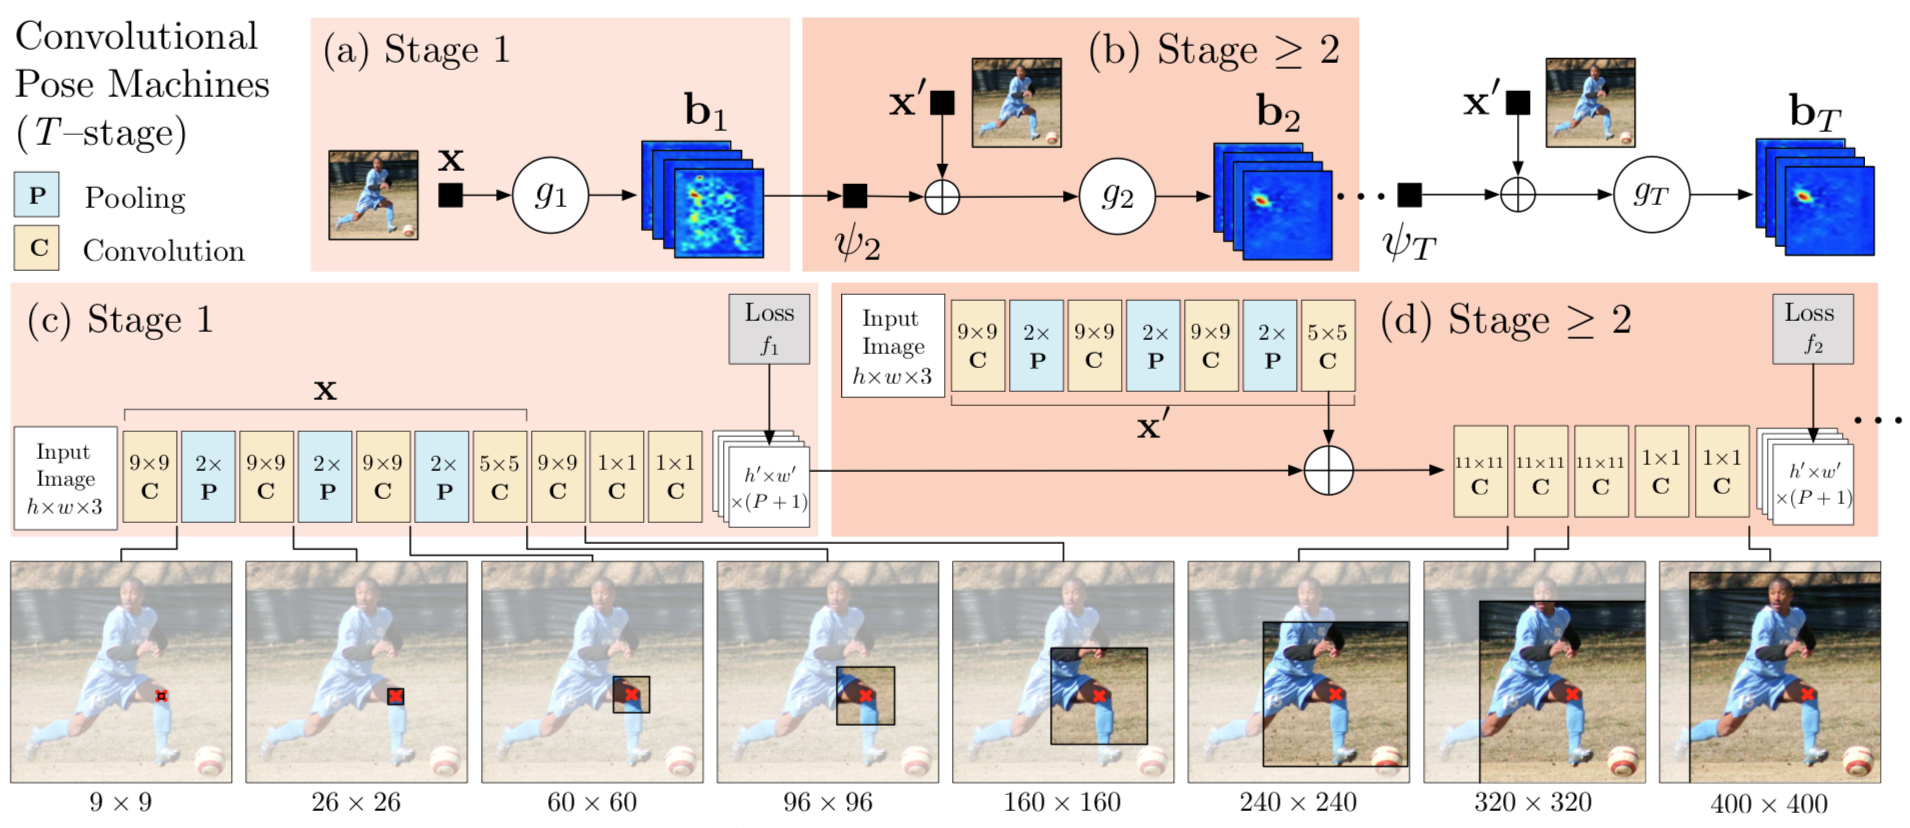
\includegraphics[width=0.9\textwidth]{./img/eft.png}
\caption{Architecture of Convolutional Pose Machines (CPMs)}\label{fig:eft}
\end{figure}
\par The belief maps provide the subsequent stage an expressive non-parametric encoding of the spatial uncertainty of location for each part, allowing the CPM to learn rich image-dependent spatial models of the relationships between parts. The overall proposed multi-stage architecture is fully differentiable and therefore can be trained in an end-to-end fashion using backpropagation\cite{Wei2016}.
\par At a particular stage in the CPM, the spatial context of part beliefs provide strong disambiguating cues to a subsequent stage. As a result, each stage of a CPM produces belief maps with increasingly refined estimates for the locations of each part.
\par In order to capture long-range interactions between parts, the design of the network in each stage of our sequential prediction framework is motivated by the goal of achieving a large receptive field on both the image and the belief maps\cite{Wei2016}.
\par Based on CPM architecture, OpenPose is an efficient method for multi-person pose estimation what uses a non-parametric representation of association scores via Part Affinity Fields (PAFs), a set of 2d vectors field that encode the location and orientation of limbs over the image domain.
\par The part affinity is a 2d vector field for each limb for each pixel in the area belonging to a particular limb, that encodes the direction that points from one part of the limb to the other . Each type of limb has a corresponding affinity field jointing its two associated body parts. A greedy parsing algorithm is sufficient to produce high-quality parses of body poses, that maintains efficiency even as the number of people in the image increase\cite{cao2017realtime}.
\par Figure \ref{fig:paf} illustrates the overall pipeline of OpenPose library.

\begin{figure}[htbp]
\centering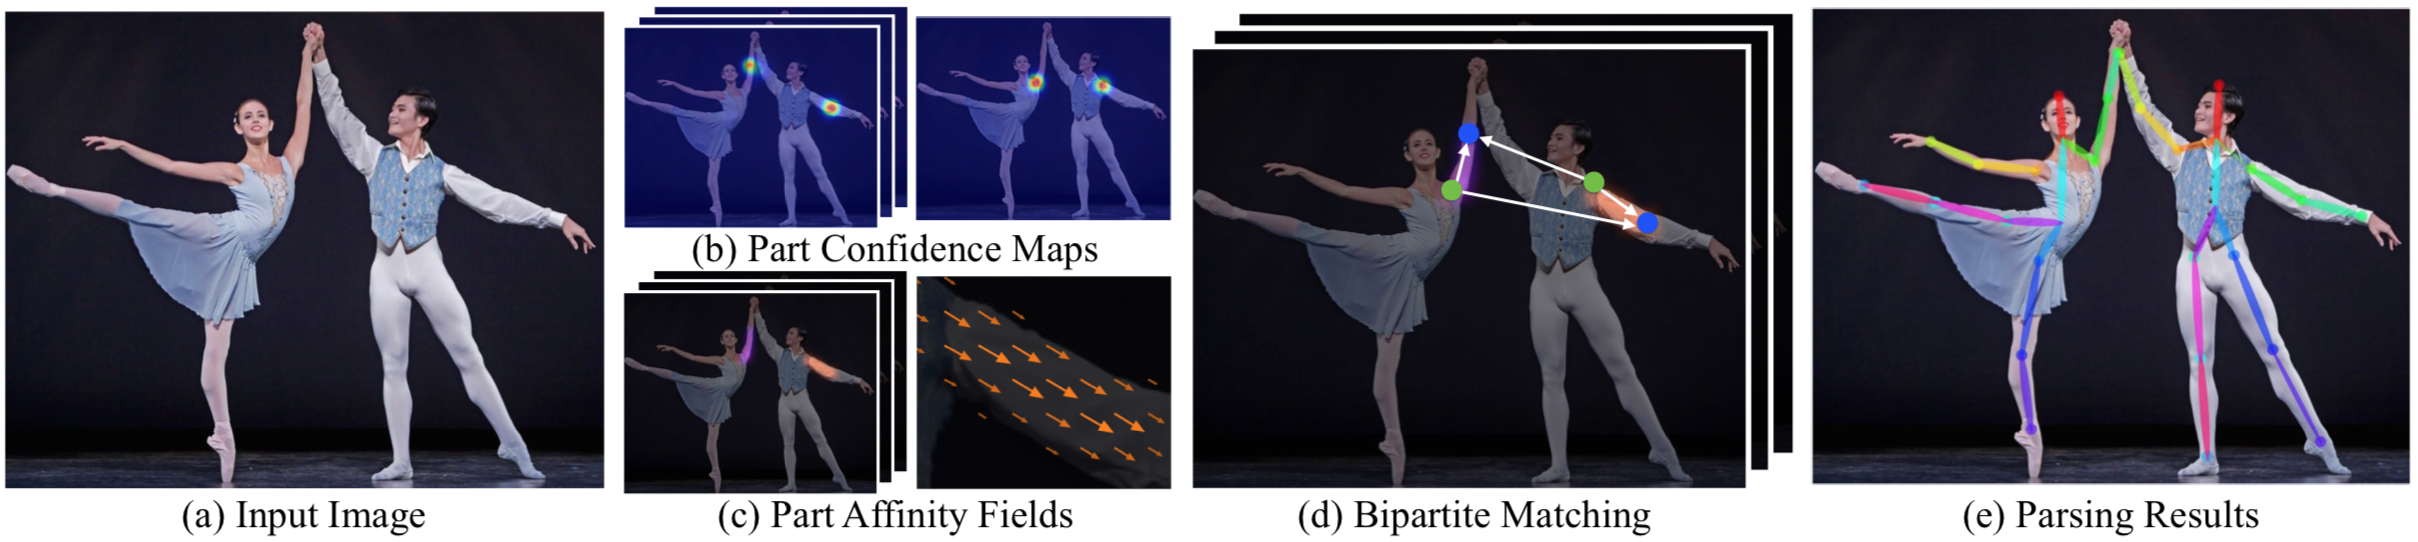
\includegraphics[scale=0.325]{./img/paf.png}
\caption{Overall pipeline of OpenPose}\label{fig:paf}
\end{figure}

\begin{itemize}
\item OpenPose takes, as input, a color image of size of $w \times h$ (Fig \ref{fig:paf}a) and produces, as output, the 2d locations of anatomical key-points for each person in the image (Fig \ref{fig:paf}e).\cite{cao2017realtime} 
\item First, a feed-forward network simultaneously predicts a set of 2d confidence maps of body part locations (Fig \ref{fig:paf}b) and a set of 2d vector fields of part affinities, which encode the degree of association between parts (Fig \ref{fig:paf}c).
\item Finally, the confidence maps and the affinity fields are parsed by greedy inference (Fig \ref{fig:paf}d) to output the 2d keypoints for all people in the image.
\end{itemize}

\begin{figure}[htbp]
\centering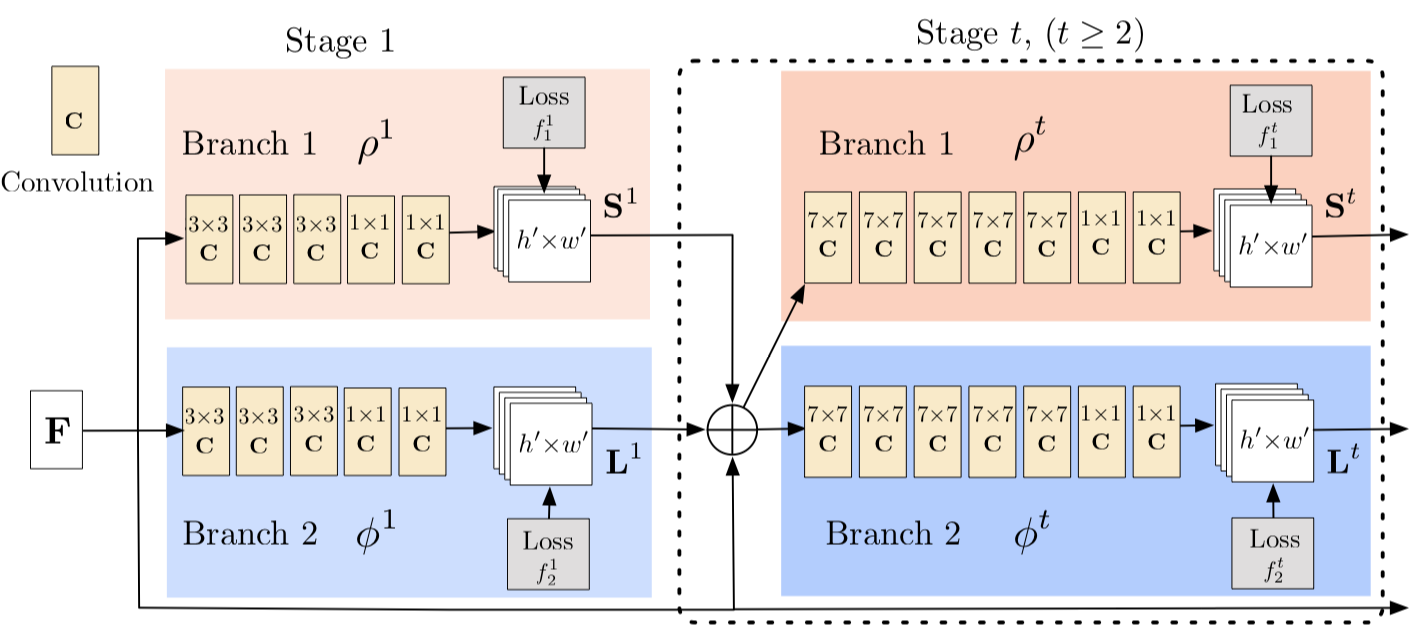
\includegraphics[width=0.9\textwidth]{./img/OpenPoseArchitecture.png}
\caption{Architecture of the two-branch multi-stage CNN in OpenPose}\label{fig:architecture}
\end{figure}

\par The architecture of OpenPose, shown in Figure \ref{fig:architecture}, simultaneously predicts detection confidence maps and affinity fields that encode part-to-part association. The network is split into two branches: the top branch, shown in beige, predicts the confidence maps, and the bottom branch, shown in blue, predicts the affinity fields. Each branch is an iterative prediction architecture, Following the typical structure of a CMP, which refines the predictions over successive stages, with intermediate supervision at each stage.

\par In our proposed system, we employed OpenPose library to extract orator's joint data from past famous 2D speech video. (Fig) We use those joint data to do template matching to get the score.

\begin{figure}[htbp]
  \centering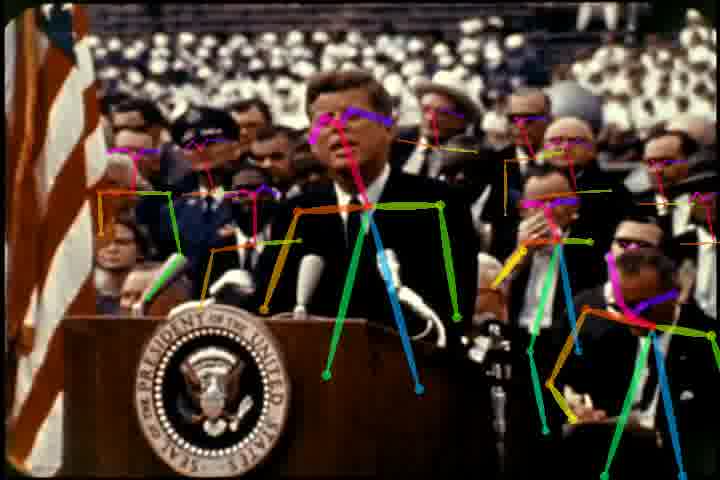
\includegraphics[width=0.9\textwidth]{./img/jfk.png}
\caption{Decocted joint by OpenPose}\label{fig:architecture}
\end{figure}



\section{Joint Data Extraction Method (3D)}
\par Recent advances in 3D depth cameras such as Microsoft Kinect sensors have created many opportunities for multimedia computing. The Kinect sensor lets the computer directly sense the third dimension (depth) of the players and the environment. It also understands when users talk, knows who they are when they walk up to it and can interpret their movements and translate them into a format that developers can use to build new experiences\cite{Zhang2012}.
\par The Kinect sensor incorporates several advanced sensing hardware. Most notably, it contains a depth sensor, a color camera, and a four-microphone array that provide full-body 3D motion capture, facial recognition, and voice recognition capabilities (see Figure \ref{fig:kinect}).
\par Figure \ref{fig:kinect}b shows the arrangement of the infrared (IR) projector, the color camera, and the IR camera. The depth sensor consists of the IR projector combined with the IR camera, which is a monochrome complementary metal oxide semiconductor (CMOS) sensor. Although the exact technology is not disclosed, it is based on the structured light principle. The IR projector is an IR laser that passes through a diffraction grating and turns into a set of IR dots\cite{Zhang2012}. 

\begin{figure}[htbp]
  \centering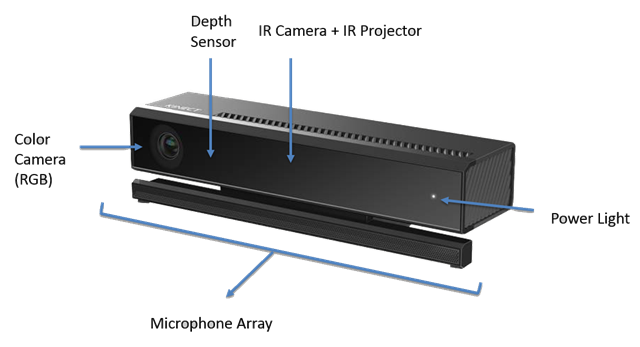
\includegraphics[width=0.9\textwidth]{./img/kinect.png}
\caption{Microsoft Kinect Sensor}\label{fig:kinect}
\end{figure}



\section{Evaluation of presentation}


\begin{table}[]
\caption{\textbf{The list of observed nonverbal cues}}
\label{my-label}
\resizebox{\textwidth}{!}{%
\begin{tabular}{llcclllccc}
\hline
\multirow{3}{*}{\#} & \multirow{3}{*}{Behaviors} & Event & \multirow{3}{*}{No.} & \multicolumn{3}{l}{Rate of occurrences} & \multicolumn{3}{c}{Percentage during observation} \\
 &  & Type &  & \multicolumn{3}{c}{(times/minute)} & \multicolumn{3}{c}{of the occurrences(\%)} \\ \cline{5-10} 
 &  & (S/P) &  & \multicolumn{1}{c}{M} & \multicolumn{1}{c}{SD} & \multicolumn{1}{c}{Range} & M & SD & Range \\ \hline
\multicolumn{10}{l}{\textbf{Postural behaviors}} \\
1 & (-) Shoulder too tight & S & 19 &  &  &  & 60.94 & 23.80 & 12.67 - 98.50 \\
2 & (-) Legs closed & S & 12 &  &  &  & 73.02 & 36.44 & 5.15 - 100 \\
3 & (-) Legs too stretch & S & 3 &  &  &  & 61.42 & 11.33 & 19.18 - 100 \\
4 & (-) Weight in on foot & S & 20 &  &  &  & 65.42 & 28.69 & 5.20 - 100 \\
5 & (-) Chin too high & S & 14 &  &  &  & 64.94 & 23.80 & 12.67 - 98.50 \\
6 & (-) Hands in pockets & S & 3 &  &  &  & 11.85 & 4.89 & 12.76 - 92.60 \\
7 & (+) Lean forward & S & 19 &  &  &  & 32.50 & 28.66 & 3.70 - 82.78 \\
8 & (-) Lean backward & S & 17 &  &  &  & 62.80 & 28.07 & 12.73 - 96.20 \\ \hline
\multicolumn{10}{l}{\textbf{Vocal behaviors}} \\
9 & (-) Speak too fast & S & 19 &  &  &  & 45.88 & 36.55 & 7.32 - 100 \\
10 & (-) Start too fast & P & 18 &  &  &  &  &  &  \\
11 & \begin{tabular}[c]{@{}l@{}}(-) Energy decreases \\       at the end\end{tabular} & P & 23 & 2.88 & 1.77 & 0.53 - 6.31 &  &  &  \\
12 & (+) Vocal emphasis & P & 33 & 5.51 & 4.51 & 0.59 - 17.50 &  &  &  \\
13 & (+) Suitable pause & P & 33 & 4.63 & 3.16 & 0.53 - 12.50 &  &  &  \\
14 & (-) Unsuitable pause & P & 20 & 1.73 & 1.14 & 0.53 - 5.19 &  &  &  \\
15 & (-) Monotone & S & 20 &  &  &  & 92.49 & 13.08 & 56.29 - 100 \\
16 & (-) Fillers & P & 34 & 5.17 & 4.22 & 1.44 - 19.03 &  &  &  \\
17 & (-) Stuttering & P & 12 & 1.72 & 0.83 & 0.53 - 3.42 &  &  &  \\ \hline
\multicolumn{10}{l}{\textbf{Behaviors of eye contact}} \\
18 & (-) Make eye contact & S & 39 &  &  &  & 93.81 & 8.24 & 75.00 - 100 \\
19 & (-) Contact avoidance & S & 28 &  &  &  & 9.98 & 8.47 & 1.12 - 25.00 \\
19.1 & (-) Look up to ceiling & S & 14 &  &  &  & 4.23 & 2.95 & 1.12 - 9.61 \\
19.2 & (-) Look down to floor & S & 19 &  &  &  & 7.67 & 4.67 & 2.84 - 14.17 \\
19.3 & (-) Look at hands & S & 11 &  &  &  & 10.24 & 3.15 & 4.40 - 13.15 \\ \hline
\multicolumn{10}{l}{\textbf{Behaviors related to facial expression}} \\
20 & (+) Facial mimicry & S & 30 &  &  &  & 39.31 & 25.97 & 4.50 - 91.81 \\
21 & (-) Smile & S & 22 &  &  &  & 13.62 & 11.54 & 3.54 - 41.08 \\
22 & (-) Flat face & S & 8 &  &  &  & 80.61 & 24.16 & 40.41 - 100 \\ \hline
\multicolumn{10}{l}{\textbf{Behaviors related to whole body movement}} \\
23 & (-) Too much movement & S & 11 &  &  &  & 42.21 & 25.97 & 4.50 - 91.81 \\
24 & (-) Too little movement & S & 23 &  &  &  & 50.62 & 29.21 & 10.05 - 100 \\
25 & (-) Step backward & P & 31 & 1.83 & 1.27 & 0.36 - 4.36 &  &  &  \\
26 & (+) Step forward & P & 34 & 2.06 & 1.04 & 0.59 - 4.61 &  &  &  \\ \hline
\multicolumn{10}{l}{\textbf{Behaviors related to hand gesture}} \\
\multicolumn{10}{l}{\textit{Amount of hand gesture}} \\
27 & Hand gesture occur & P & 38 & 16.83 & 7.15 & 0.93 - 28.42 &  &  &  \\
28 & (-) Too little gestures & S & 20 &  &  &  & 69.55 & 34.64 & 17.21 - 100 \\
29 & (-) Too much gestures & S & 10 &  &  &  & 61.49 & 31.82 & 27.34 - 96.10 \\ \hline
\multicolumn{10}{l}{Quality of hand gestures} \\
30 & (-) Bounded gestures & P & 30 & 6.75 & 5.33 & 1.00 - 19.77 &  &  &  \\
31 & (+) Relaxed gestures & P & 29 & 7.41 & 4.95 & 1.15 - 15.79 &  &  &  \\
32 & (-) Casual gestures & P & 10 & 5.16 & 3.14 & 1.56 - 10.28 &  &  &  \\
33 & (-) Uncompleted gesture & P & 27 & 3.23 & 2.78 & 0.93 - 10.27 &  &  &  \\
34 & (+) Gestural emphasis & P & 20 & 4.43 & 4.05 & 0.36 - 11.99 &  &  &  \\
35 & (-) Repeated gestures & P & 31 & 6.57 & 2.49 & 1.09 - 12.31 &  &  &  \\ \hline
\end{tabular}%
}
\end{table}

